\section{绪论}

\subsection{选题背景}
互联网技术的蓬勃发展在很大程度上给人们的生活带来了越来越多的便利,人们在逐渐适应网络这样的平台的同时,也更倾向于甚至依赖在网络平台上完成生活中的各种事情,可以说,网络对于人们的重要性已经几乎等同于空气、水和食物。按照网络平台的功能来划分,门户网站(新浪、搜狐等)是新闻实事评论发布的主要渠道,社交网站(微博、人人等)是人们分享个人想法和心情的首选,博客系统(新浪博客、百度空间等)是人们发表和传达思想和经验的主要平台,以及一些新新涌现的图片和视频等多媒体资源分享平台(优酷土豆、POCO等)大大丰富了人们的娱乐生活。此外,鉴于国内发达的物流行业,各大电子商务平台(淘宝、京东等)也使得不用出门就能购物成为了现实。按照网络平台资源的载体来划分,包括文本、图片、音乐和视频几大类,其中文本无疑是整个互联网资源的主体,无论是传统的新闻、博客、评论、说明,还是新新发展的弹幕视频网站(Acfun\footnote{http://www.acfun.tv/}、Bilibili\footnote{http://www.bilibili.com/}等),都是由很多文本信息组成的。按照网络平台的用户参与角度来划分,可以将用户角色分为两种:信息发布者和信息获取者。以程序员为例,当他需要学习一项新技术时,往往会通过搜索引擎寻找一些与该技术相关的教学经验文章,从而使自己尽快掌握该项技术。等对该技术数量掌握之后,往往又会通过写技术博客的方式记录下他的学习历程和使用中的经验之谈,以供他人参考。同时,该用户还肯定拥有其他多个兴趣爱好,比如他可以与网上其他用户分享旅游游记、摄影作品等等。

虽然这些网站系统在功能上、信息载体上或是用户参与方式上都截然不同,但是宏观来看他们都存在一个共同的问题:信息孤岛现象。如图\ref{fig:problem}所示,当这些网站发展越来越多之时,各个网站之间信息不流通的问题也日渐明显,每个网站独立发展,出于安全性等方面的考虑,其资源和用户的数据并不能实现跨平台共享,从而使得每个网站成为一座座信息孤岛。

\begin{figure}[ht]
\centering
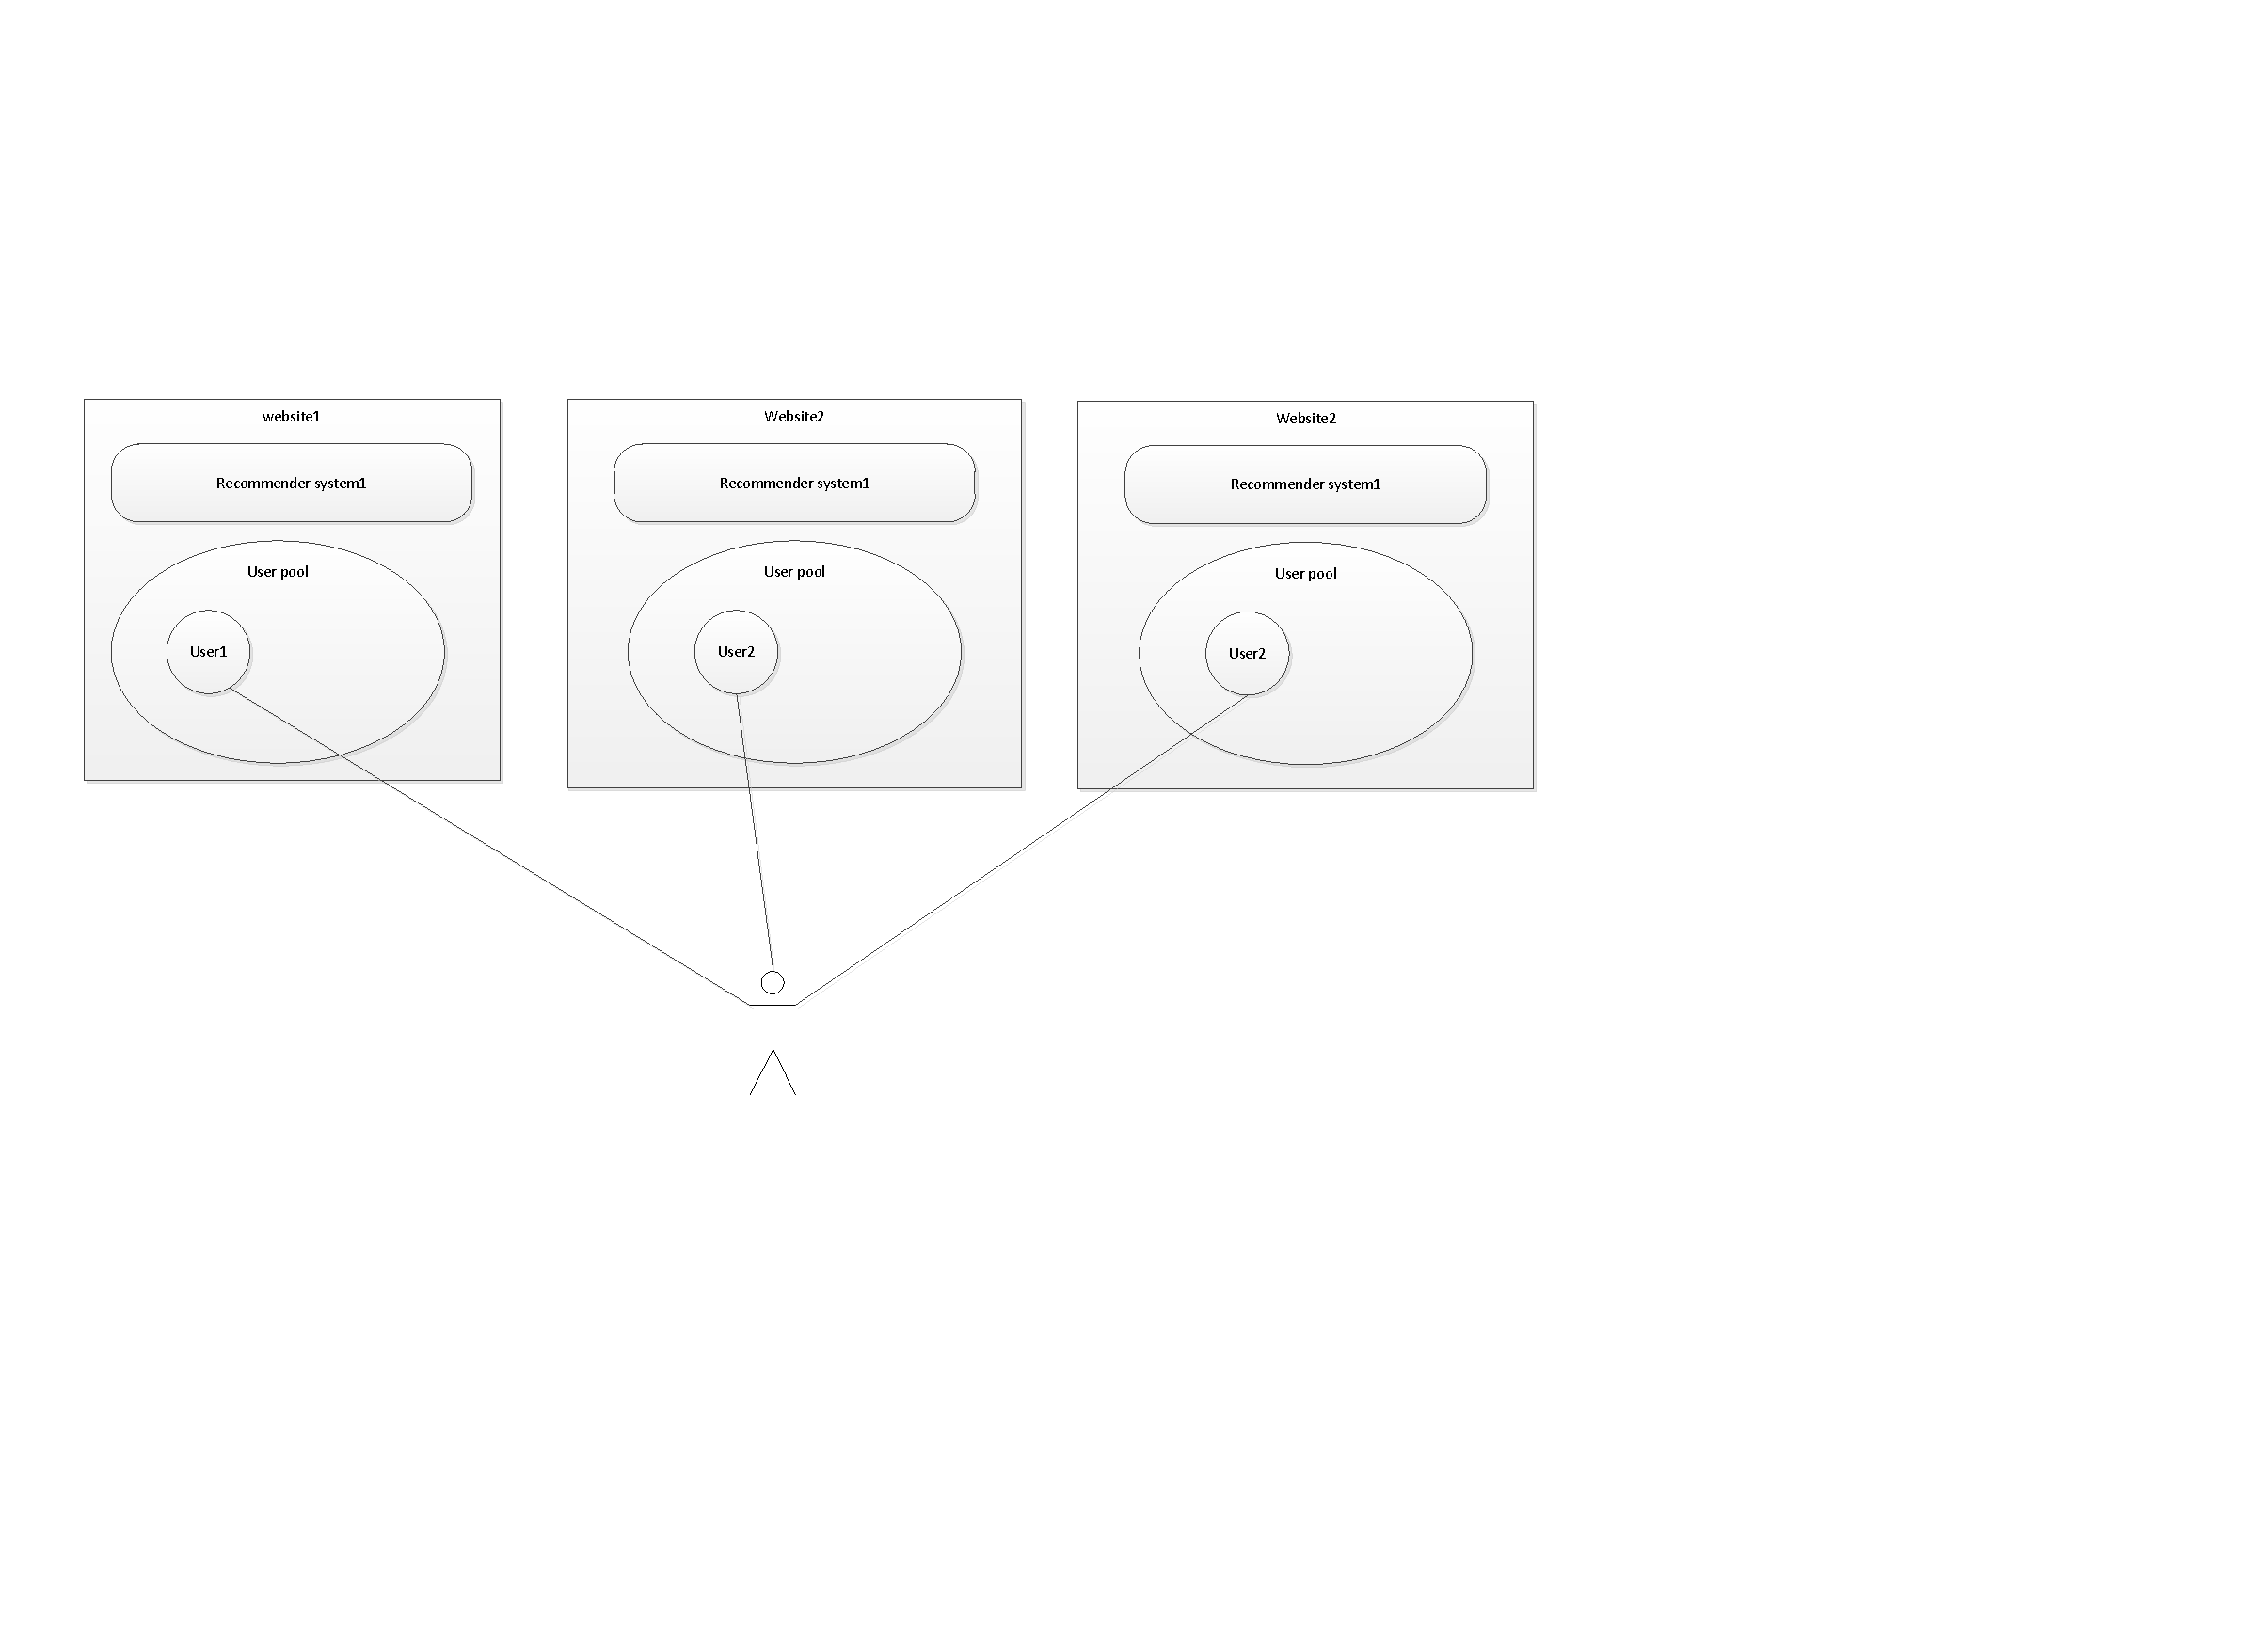
\includegraphics[width=\textwidth]{problem.pdf}
\caption{互联网平台的信息孤岛现象}
\label{fig:problem}
\end{figure}

举例来说,当用户作为信息获取者时,虽然每个网站可以为本平台上的用户提供很好的用户体验,通过数据挖掘等技术发现用户的兴趣,为其推荐有潜在需求的信息,但是不同网站之间的用户兴趣不能共享,导致兴趣推荐的不准确。当用户作为信息发布者时,其操作会更加繁琐,他往往需要打开多个网站重复几乎相同的操作来发布同样的内容,最明显的证据就是同时使用微信、微博和人人的用户需要在三个平台上重复三次操作完成发布。当这些网站越来越多的时候,问题也随之而来,即用户可能需要打开很多个独立的网站来完成一系列类似的事情。比如,先在新闻网站上浏览最新发生的时事,接着在摄影网站上发布新照片,然后在社交网站上浏览好友更新的状态,最后在电商网站上购买一些商品等等。换句话说,用户是单向地去寻找想要的信息,这其中无疑包含了一些不必要的重复操作。退一步来说,即使存在某些用户只在社交网站上浏览信息,很少接触其它网站,也会有一些重复操作的问题。因为该用户的好友很有可能是分散地活跃于各个不同的社交网站平台(微博、人人网等),而且每个平台发布的信息肯定有所不同,所以该用户仍然需要逐个登录各个网站后才能浏览到各个用户的信息。再退一步说,即便现在已经有些软件把所有社交网站整合成一个统一接口,让用户只需一次登录就能同时访问多个平台,用户仍然会遇到信息冗余的问题,比如重复的新闻、不感兴趣的推荐等等。

为了解决上述问题,我们设想有这样一个智能系统:每当用户打开系统时,系统会自动推送今天的时事新闻、其好友最近更新的状态、感兴趣或者正在促销的商品,以及一些根据用户偏好过滤的信息。此外,他也可以在系统上发布自己的信息给他的好友,甚至给那些对他信息感兴趣的陌生人。虽然,实现这样一个系统的工作量和难度是巨大的,但仔细观察后可以发现这样一个重要的规律:即用户希望所有的信息能够在整个互联网上智能地自主流动,在用户单方面寻找信息的同时,让信息也能自主地流向符合特定需求的用户。

\begin{figure}[ht]
\centering
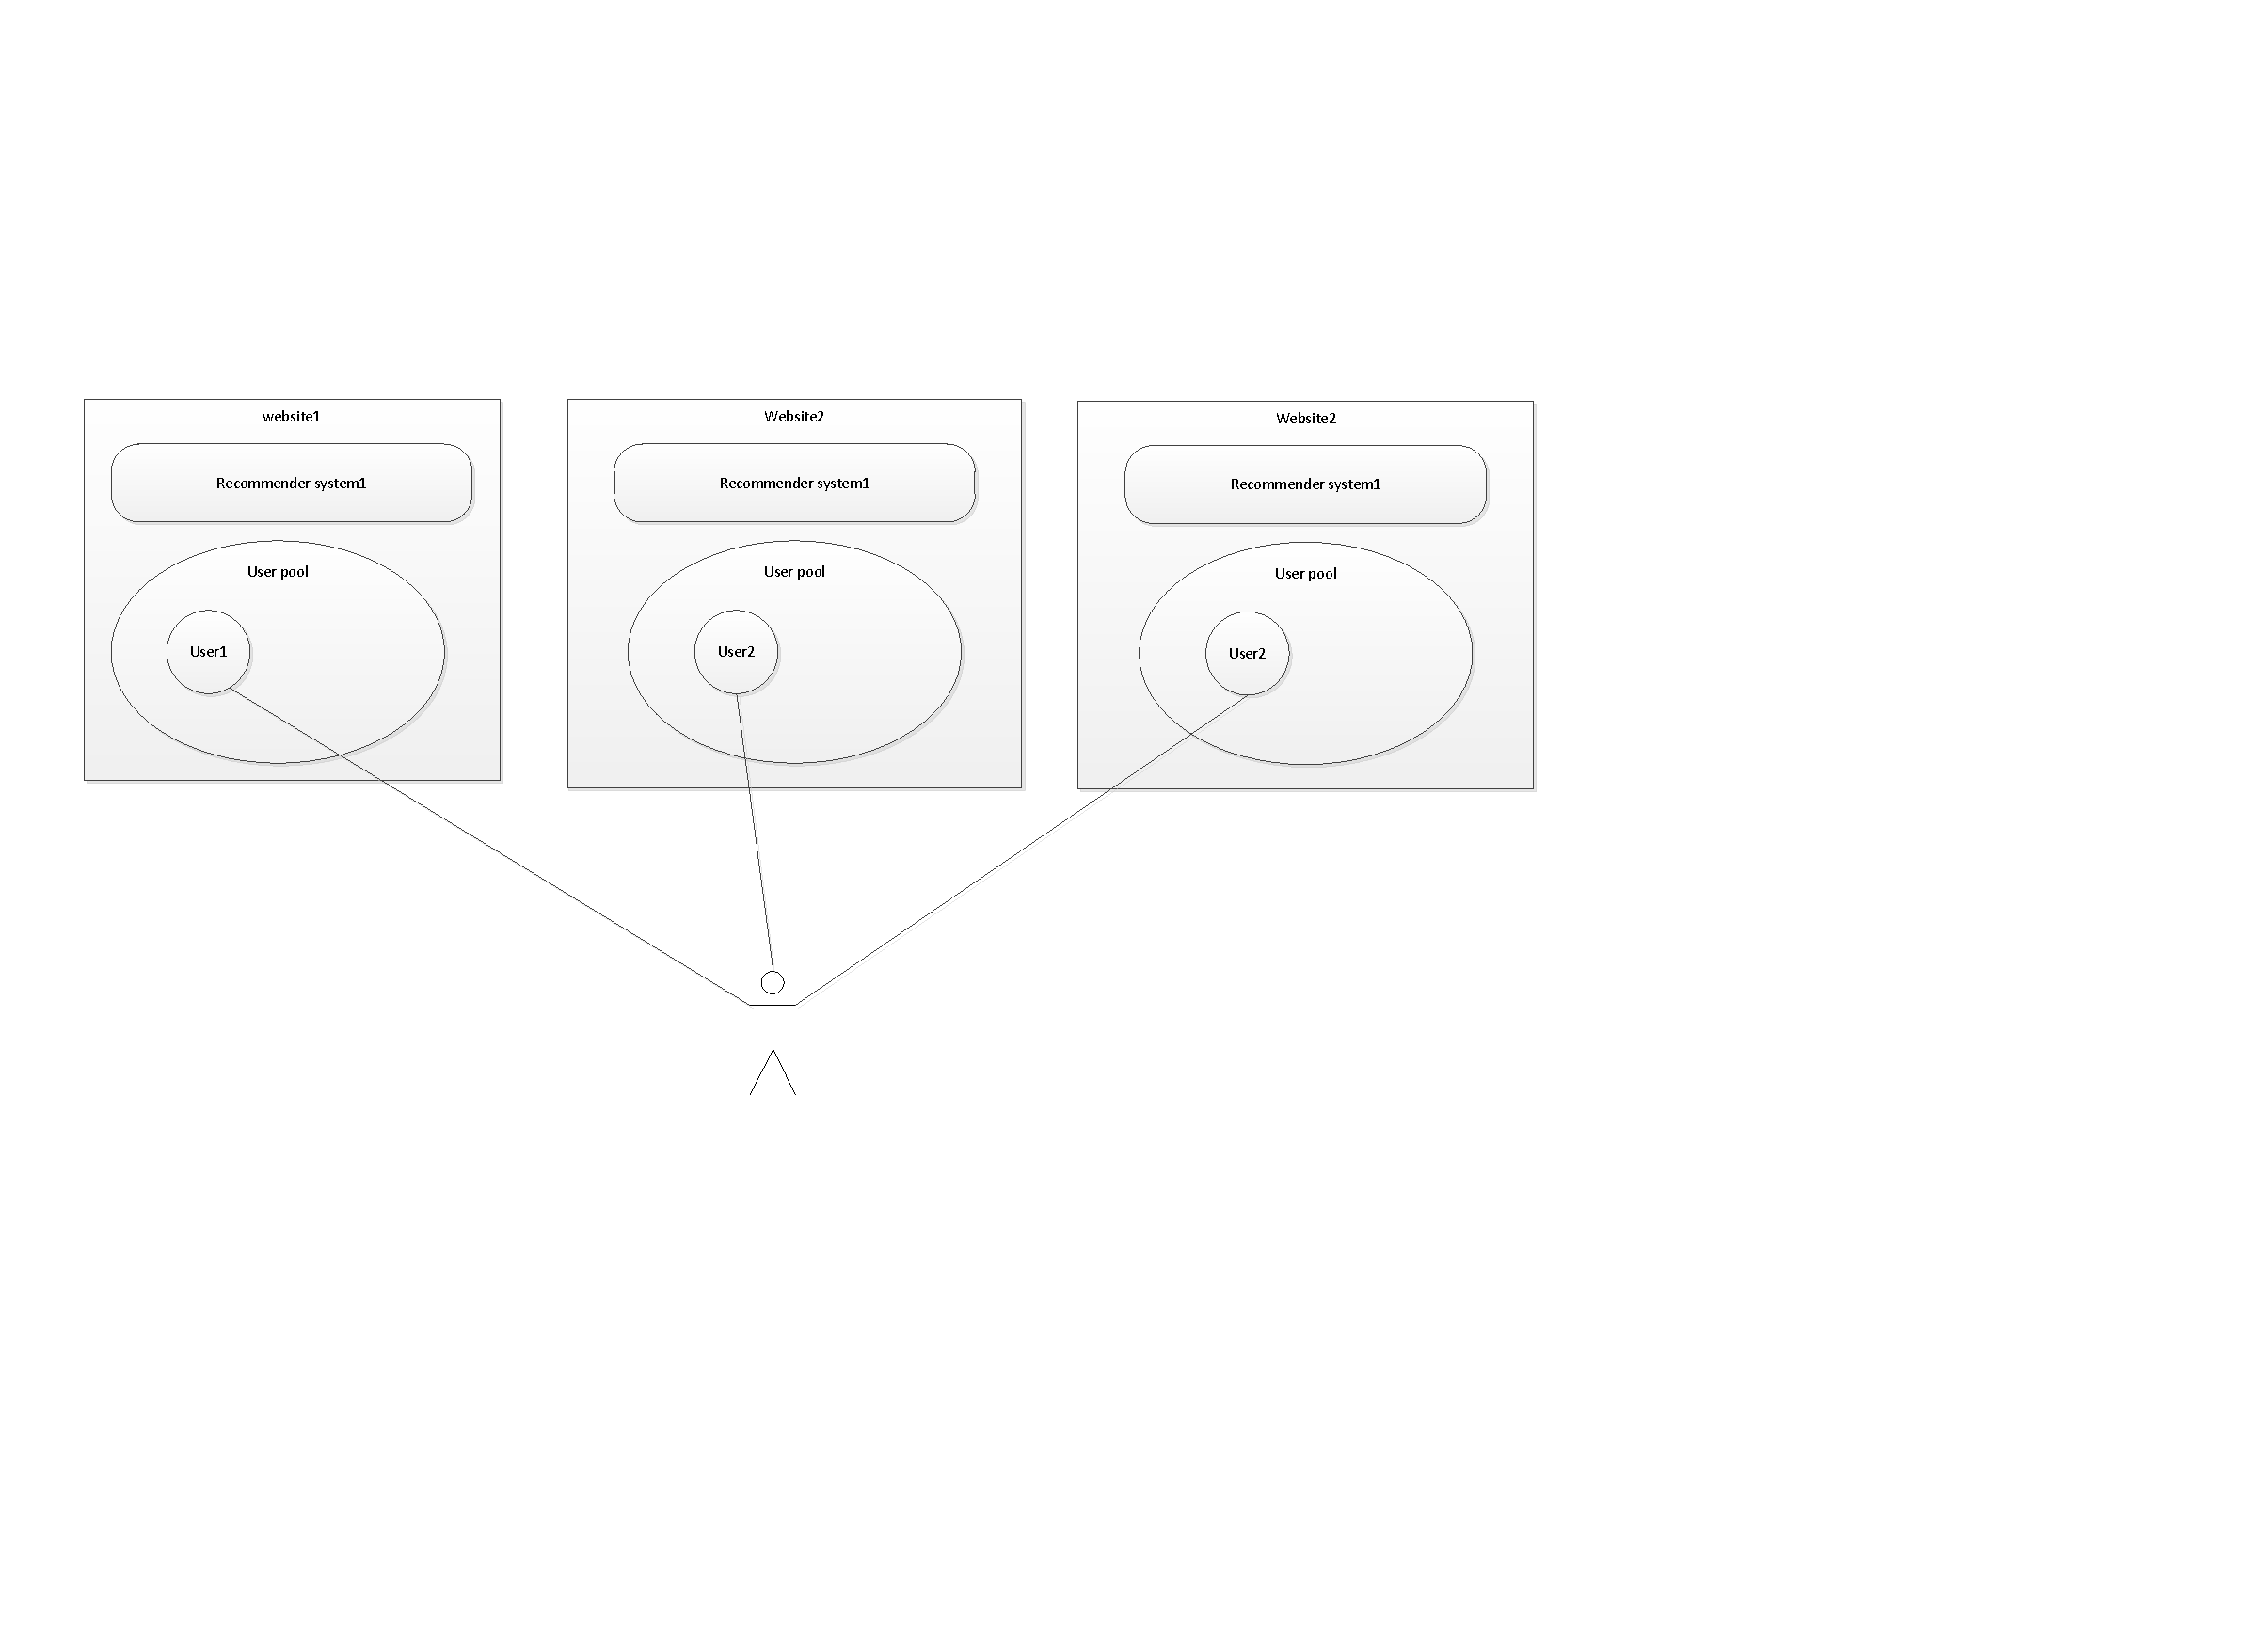
\includegraphics[width=\textwidth]{problem.pdf}
\caption{基于P2P网络的智能系统架构}
\label{fig:solution}
\end{figure}

从抽象层面来看,要实现这样一套信息自主流动的机制,传统的集中式计算模式已经不再适用。如图\ref{fig:solution}所示,这里每个用户均看作一个独立的节点,所有的节点整合在一起就形成一个巨大的P2P网络。其中,每个节点既充当服务器用于分发信息,也充当客户端用于接收信息,并且由某个节点发出的信息在其它节点间传播的时候会自主流动,寻找潜在的、匹配的节点。简单来说,要使信息能够自主流动,就要解决这样几个问题:

\begin{itemize}
\item 资源信息描述与匹配:互联网资源普遍呈现出半结构化或非结构化的特征,例如普通的新闻或者博客,除开诸如作者、标题、时间等结构化信息,正文纯文本就是典型的非结构数据。因此
\item 用户兴趣挖掘与关联:
\item P2P网络路由与搜索:
\end{itemize}

\subsection{研究意义与应用价值}
总结起来可以发现各个互联网平台之间相互封闭而导致的信息孤岛现象存在一下几个问题:

\begin{itemize}
\item 从计算资源的角度来看,在P2P网络架构中,每个节点都可以既可以充当服务器为其它节点提供资源,也可以作为客户端向其它节点获取资源。从而使得硬件资源得到充分地利用,而不是像中心化架构中的服务器一样存在计算瓶颈。
\item 从隐私安全的角度来看,所有的用户数据都存储在本地。
\item 从拓扑架构的角度来看,扩展性好,。。。。
\end{itemize}

\subsection{国内外研究现状}

\subsection{本文研究内容}

\subsection{本文内容安排}

